\section{Initializing states with enhanced coherence by adiabatic transition}
\label{sec:adiabatic_transition}

The preceding sections identified drive parameters that render a pair of cavity-like Floquet states robust against flux fluctuations. In practice, however, the system is initialized in the computational basis of the static Hamiltonian rather than in these dressed Floquet states. This section describes how to transfer population from the bare computational states to the target Floquet states via an adiabatic ramp of the drive amplitude.

In the adiabatic frame, we introduce a time-dependent unitary transformation \(U(\Omega_t)\) that diagonalizes the instantaneous Hamiltonian \(H(\Omega_t)\). The corresponding effective Hamiltonian is
\begin{equation}
\begin{aligned}
H_{\mathrm{eff}}(\Omega_t)
&= U^\dagger(\Omega_t)\!\left( H(\Omega_t) - i\hbar \frac{\partial}{\partial t} \right)\!U(\Omega_t) \\
&= H_d(\Omega_t) + V(\Omega_t).
\end{aligned}
\end{equation}

The diagonal part \(H_d\) contains the instantaneous energy eigenvalues \(E_j(\Omega_t)\):
\begin{equation}
H_d(\Omega_t)=\sum_j E_j(\Omega_t)\,|j\rangle\langle j|.
\end{equation}
The coupling term \(V\) originates from the induced gauge contribution \(i\hbar\,U^\dagger \dot U\) and captures the effect of the time-dependent driving. Splitting \(V\) into off-diagonal and diagonal components gives
\begin{equation}
\begin{aligned}
V
&=
\underbrace{-i\hbar \sum_{j\neq j'} 
\frac{\langle j'|\,U^\dagger \dot H\,U\,|j\rangle}{E_j-E_{j'}}\,|j'\rangle\langle j|}_{V_{od}}
\\
&\quad+\;
\underbrace{-i\hbar \sum_j \langle j|\,U^\dagger \dot U\,|j\rangle\,|j\rangle\langle j|}_{V_d}.
\end{aligned}
\end{equation}
where the diagonal terms contribute to the Berry phase, while the off-diagonal terms drive transitions.

In our case of interest, the goal is to adiabatically evolve into the desired Floquet states. When counter-rotating terms are negligible, this evolution is equivalent to adiabatic dynamics governed by the rotating-frame Hamiltonian
\begin{equation}
\begin{aligned}
H_R(t) =\;&
\Delta_{bd}\, b^\dagger b
+ \frac{K}{2}\, b^{\dagger 2} b^{2}
+ \overline{\omega}_c\, c^\dagger c \\
&+ \chi\, b^\dagger b\, c^\dagger c
+ \Omega_I(t)\, ( b + b^\dagger ) .
\end{aligned}
\end{equation}

Under the drive $\Omega_I(t)$, the Hamiltonian in the instantaneous eigenbasis can be written as
$H_{\mathrm{eff}} = H_d(\Omega_I) + V(\Omega_I)$.
For the driven operating regime of interest, the diagonal contribution is well approximated by Eq.\ \eqref{eq:Hd_far_detuned}
\begin{equation}
\begin{aligned}
H_d(\Omega_I) \approx\;&
\left( \Delta_{bd} - \frac{\Omega_I^2}{\kappa} \right) \sigma^+ \sigma^-
+ \left( \tilde{\omega}_c + \frac{\Omega_I^2 \chi}{\Delta_{bd}^2} \right) c^\dagger c \\
&+ \chi \left( 1 - 2 \frac{\Omega_I^2}{\Delta_{bd}^2} \right) \sigma^+ \sigma^-\, c^\dagger c .
\end{aligned}
\end{equation}

Nonadiabatic leakage is generated by the time dependence of the drive through the off-diagonal term $V_{od}$.
In particular,
\begin{equation}
U^\dagger \dot{H}_R U
= \dot{\Omega}_I\, U^\dagger (b^\dagger + b) U
\approx \dot{\Omega}_I\, \sigma_x
+ \mathcal{O}\!\left(\frac{\dot{\Omega}_I}{\Delta_{bd}}\right).
\end{equation}
which yields the effective coupling between $|g\rangle$ and $|e\rangle$,
\begin{equation}
V_{od}(\Omega_I) \approx \frac{\dot{\Omega}_I}{\Delta_{bd}}\, \sigma_y .
\end{equation}

Suppressing leakage requires the nonadiabatic coupling to remain small compared to the instantaneous gap,
\begin{equation}
\frac{\dot{\Omega}_I}{\Delta_{bd}} \ll \Delta_{bd}.
\end{equation}
For a ramp of characteristic amplitude $\Omega_0$ executed over a ramp time $\tau$ (so that $\dot{\Omega}_I \sim \Omega_0/\tau$), this implies the lower bound
\begin{equation}
\tau \gg \frac{\Omega_0}{\Delta_{bd}^2}\overset{\eqref{eq:ss_unselective}}{=}\sqrt{\frac{1}{4K\Delta_{bd}}}.
\end{equation}
Increasing $\Delta_{bd}$ can reduce $\tau$ to obtain the desired state.

To bypass this speed limit, we implement a shortcut to adiabaticity using an active quadrature control field $\Omega_Q$ which is DRAG-style.
Specifically, we augment the drive Hamiltonian by
\begin{equation}
H_{\text{total}} = H_R - i \Omega_Q (b - b^\dagger),
\end{equation}
and choose the quadrature amplitude to cancel the nonadiabatic coupling,
\begin{equation}
\Omega_Q = -\frac{\dot{\Omega}_I}{\Delta_{bd}}.
\end{equation}
The effective Hamiltonian in the adiabatic frame then becomes
\begin{equation}
\begin{aligned}
&U^\dagger \left( H_R - i \Omega_Q (b - b^\dagger) - i \frac{\partial}{\partial t} \right) U\\
&\approx H_d + V_d + \frac{\dot{\Omega}_I}{\Delta_{bd}} \sigma_y - \frac{\dot{\Omega}_I}{\Delta_{bd}} \sigma_y \\
&= H_d + V_d,
\end{aligned}
\end{equation}
so the evolution remains diagonal in the instantaneous eigenbasis even for fast ramps.

Numerical simulations confirm the qualitative analysis above. We compute the state-preparation infidelity at the end of the ramp as a function of the ramp time $\tau$ for several detunings $\Delta_{bd}$.
The infidelity is defined as the average loss of overlap with the target Floquet states,
\begin{equation}
\label{eq:infidelity_def_ch7}
\mathcal{I}(\tau)
=
1-\frac{1}{2}\left[
\mathrm{Tr}\!\left(P_{g0}(\tau)\,\bar{\mathcal{E}}_{\tau}\!\left(\rho_{0,g0}\right)\right)
+
\mathrm{Tr}\!\left(P_{g1}(\tau)\,\bar{\mathcal{E}}_{\tau}\!\left(\rho_{0,g1}\right)\right)
\right].
\end{equation}
where $P_{g0}(\tau)=|\phi_{g0}(\tau)\rangle\langle\phi_{g0}(\tau)|$ and
$P_{g1}(\tau)=|\phi_{g1}(\tau)\rangle\langle\phi_{g1}(\tau)|$ project onto the desired Floquet states at the end of the pulse. The map
$\bar{\mathcal{E}}_{\tau}(\cdot)=\langle \mathcal{E}_{\tau}^{\delta\Phi}(\cdot)\rangle_{\delta\Phi}$
denotes the evolution averaged over flux trajectories $\delta\Phi(t)$, with each trajectory generated by the master equation Eq.\ \eqref{eq:lindblad_full_ch8}.
The initial states are
$\rho_{0,g0}=|\bar g0\rangle\langle\bar g0|$ and
$\rho_{0,g1}=|\bar g1\rangle\langle\bar g1|$, where the overbar denotes eigenstates of the static system Hamiltonian in the dispersive regime.

Results are shown in Fig.~\ref{fig:ramp}. For a fixed detuning, the infidelity initially decreases with increasing $\tau$ because a slower ramp improves adiabaticity and suppresses coherent leakage, but it eventually increases as the longer evolution accumulates more decoherence error. For a fixed ramp time (e.g., $\tau=50\,\mathrm{ns}$), larger detuning yields lower infidelity, due to larger instantaneous gap. Finally, for the same detuning and ramp time, DRAG outperforms a Gaussian ramp because the added $Q$-quadrature control enhances adiabaticity by suppressing unwanted transitions.

\begin{figure}[H]
    \centering
    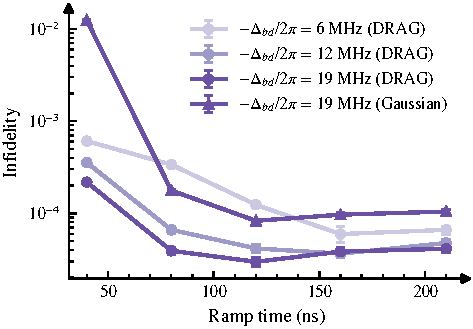
\includegraphics[width=\linewidth]{chapter7/figures/preparation_fidelity_plot.pdf}
    \caption{State-preparation infidelity $\mathcal{I}(\tau)$ versus ramp time $\tau$ for several detunings $\Delta_{bd}$, comparing Gaussian and DRAG ramps. The non-monotonic dependence reflects the trade-off between coherent leakage from unwanted transitions (suppressed for longer $\tau$) and decoherence (which accumulates for longer $\tau$).}
    \label{fig:ramp}
\end{figure}
